\documentclass[a4paper,slidestop,xcolor=pst,blue]{beamer}

\input{slidesHeader.tex}

\title[Capa de Servicio - Fundamentos]{Capa de Servicio - Fundamentos }

\author[P. S{\'a}nchez]{\alert{Pablo S{\'a}nchez}}

\institute[IIE]{
		   Dpto. Ingenier{\'i}a Inform{\'a}tica y Electr{\'o}nica \\
		   Universidad de Cantabria \\
		   Santander (Cantabria, Espa{\~n}a) \\
		   \texttt{p.sanchez@unican.es}
}

\date{}

\begin{document}

\begin{frame}[c]
	\titlepage
	\begin{columns}
		\column{0.50\linewidth}
			\centering
    		\includegraphics[width=.28\textwidth,keepaspectratio=true]{images/istr.eps}
		\column{0.50\linewidth}
			\centering
			\includegraphics[width=.25\textwidth,keepaspectratio=true]{images/uc.eps}
	\end{columns}
\end{frame}

\begin{frame}[c]
    \frametitle{\alert{Advertencia}}
    \begin{center}
        Todo el material contenido en este documento no constituye en modo alguno una obra de referencia o apuntes oficiales mediante el cual se puedan preparar las pruebas evaluables necesarias para superar la asignatura. \ \\
        \ \\
        Este documento contiene exclusivamente una serie de diapositivas cuyo objetivo es servir de complemento visual a las actividades realizadas en el aula para la transmisi{\'o}n del contenido sobre el cual versar{\'a}n las mencionadas pruebas evaluables.  \ \\
        \ \\
        Dicho de forma m{\'a}s clara, \alert{estas transparencias no son apuntes y su objetivo no es servir para que el alumno pueda preparar la asignatura.}
    \end{center}
\end{frame}

\section{Introducción}

\begin{frame}[t]
    \frametitle{Capa de Servicio}
    \only<1|handout:0>{
        \rput[lt](-0.2,0){
            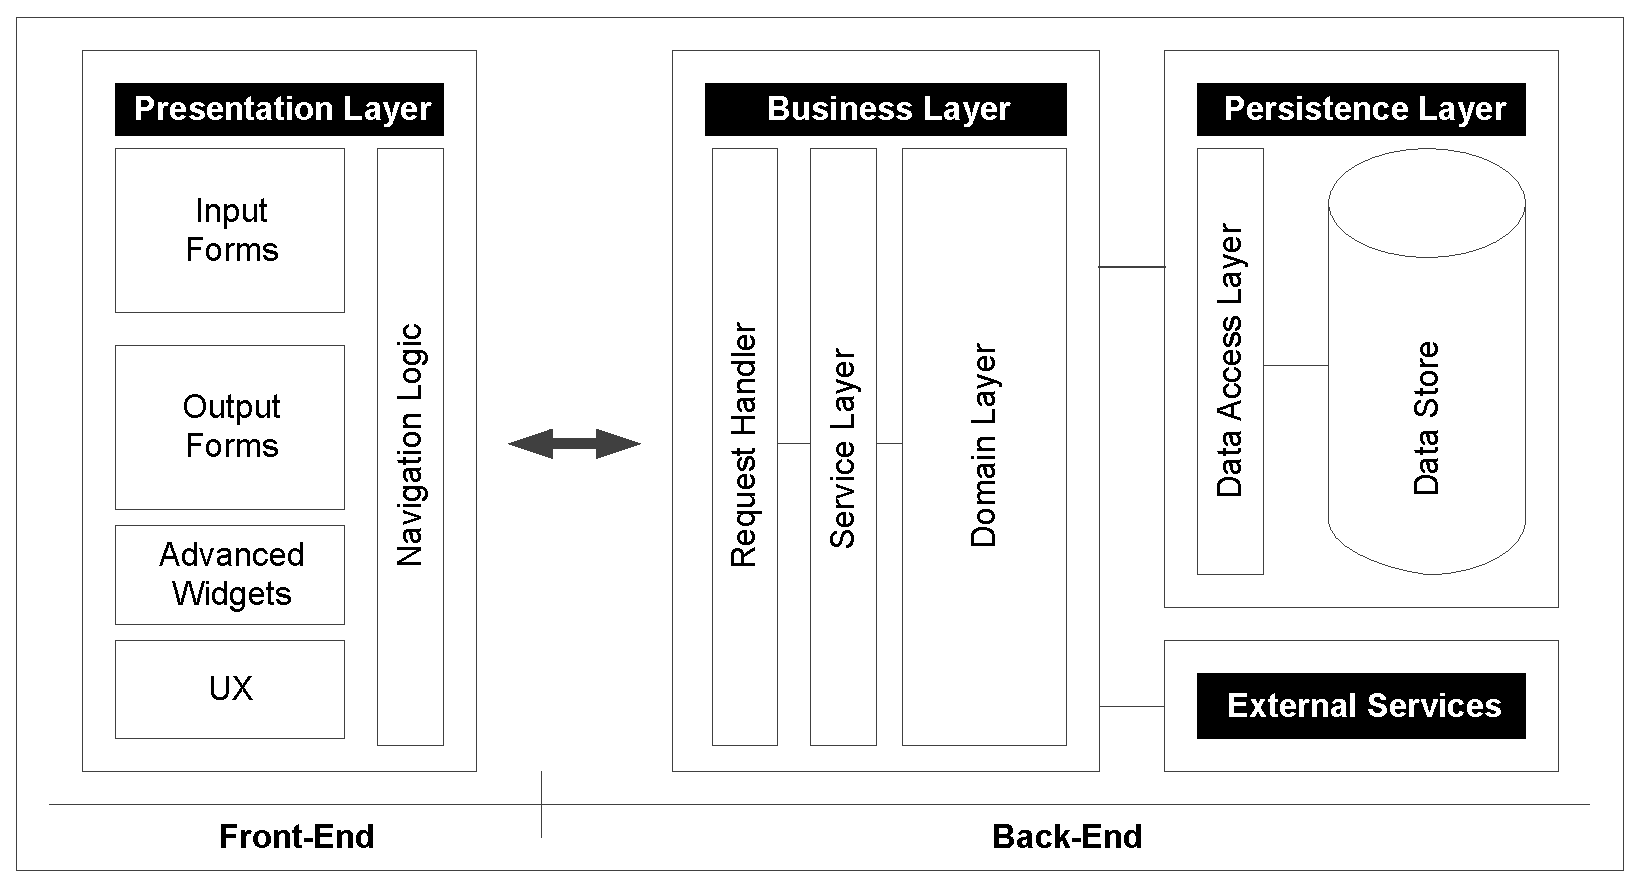
\includegraphics[width=\linewidth]{images/intro/enterpriseArchitectures00.eps}
        }
    }
    \only<2|handout:1>{
        \rput[lt](-0.2,0){
            \includegraphics[width=\linewidth]{images/intro/enterpriseArchitectures01.eps}
        }
    }
\end{frame}

\begin{frame}[c]
	\frametitle{Responsabilidades de la Capa de Servicio}
	\begin{enumerate}[<+->]
        \item Atender las peticiones HTTP de los clientes, delegando en el modelo de dominio.
        \item Asegurar la transaccionalidad de las operaciones de negocio.
        \item Validar las peticiones de los clientes.
        \item Recuperar y almacenar datos del almacén o almacenes persistentes.
        \item Facilitar la eficiencia del sistema.
        \item Controlar el acceso a los datos.
        \item Gestionar la comunicación con los servicios externos.
        \item Gestionar de manera adecuada casos excepcionales.
        \item Ayudar a satisfacer los requisitos no funcionales.
	\end{enumerate}
\end{frame}

\begin{frame}[c]
    \frametitle{Objetivos del Tema}
    \begin{enumerate}[<+->]
         \item Comprender en profundidad cuáles son las responsabilidades de la capa de servicio.
         \item Comprender cómo funciona el protocolo HTTP.
         \item Comprender los principios de las arquitecturas REST.
         \item Saber diseñar una API REST.
         \item Ser capaz de usar los patrones de diseño propios del diseño de una capa de servicio.
    \end{enumerate}
\end{frame}

\begin{frame}[c]
    \frametitle{Bibliografía}
    \begin{thebibliography}{1}

        \bibitem[Fowler, 2002]{Fowler2002}
        Fowler, M. (2002).
        \newblock {\em {Patterns of Enterprise Application Architecture}}.
        \newblock Addison-Wesley.

        \bibitem[Esposito and Saltarello, 2014]{Esposito2014}
        Esposito, D. y Saltarello, A. (2014).
        \newblock {\em {Microsoft .NET - Architecting Applications for the
          Enterprise}}. 2ª Ed..
        \newblock Microsoft Press

        \bibitem{Ricahrdson2007}
        Richardson, L. and Ruby, S.
        \newblock {\em {RESTful Web Services}}.
        \newblock  O'Reilly, 2007.

    \end{thebibliography}
\end{frame}

\section{Arquitecturas REST}

\subsection{Arquitecturas REST}

\begin{frame}
    \frametitle{Arquitecturas REST}
    \begin{center}
        \includegraphics[width=\linewidth]{images/rest/enterpriseArchitectures(rest).eps}
    \end{center}
\end{frame}

\begin{frame}[c]
	\frametitle{Arquitectura REST}
    \begin{block}{REST \emph{(REpresentational State Transfer)}}
        \begin{enumerate}[<+->]
            \item  REST es un estilo arquitectónico diseñado para satisfacer las necesidades de los sistemas de hipermedia a escala de internet.
            \item Un \emph{sistema hipermedia} se concibe como una máquina de estados donde el usuario progresa mediante la selección de enlaces y el envío de formularios.
            \item La representación de cada estado se transfiere al usuario.
        \end{enumerate}
    \end{block}
    \uncover<4->{
    	\begin{block}{Sistema Hipermedia}
            Un \emph{sistema hipermedia} es un sistema que fusiona información de control de la aplicación con la presentación de su información. La información se puede presentar utilizando diversos formatos, tales como texto, gráficos, audio o vídeo.
    	\end{block}
    }
\end{frame}

\begin{frame}[c]
	\frametitle{Objetivos Arquitectura REST}
    \begin{enumerate}[<+->]
        %% Enlaces
        \item Minimizar latencias.
        %% Escalabilidad
        \item Minimizar comunicaciones a nivel de red.
        %% Altas cargas de usarios
        \item Maximizar la escalabilidad de los componentes.
        \item Maximizar la independencia de los componentes.
        \item Permitir almacenar en cachés resultados e interacciones.
        \item Permitir la sustitución dinámica de componentes.
        \item Permitir el procesamiento de acciones por intermediarios.
    \end{enumerate}
\end{frame}

\begin{frame}[c]
	\frametitle{Estilos Arquitectura REST}
    \begin{enumerate}[<+->]
        %% Presentación vs Almacenamiento y Procesamiento.
        %% Portabilidad
        %% Reemplazabilidad dinámica de comportamiento.
        \item Cliente-Servidor.
        %% El servidor no debe almacenar nada sobre el estado de los clientes.
        %% Cada petición del cliente debe tener toda la información necesaria para interpretarla.
        %% Favorece la escalabilidad.
        %% Favorece reliability (puedo volver a un estado anterior)
        %% Favore procesamiento por terceros.
        \item Sin estado.
        %% Favorece el rendimiento
        \item Respuestas cacheables.
        %% Favorece la evolución
        %% Favorece la visibilidad
        \item Interfaces uniformes entre componentes.
        \item Código bajo demanda (opcional).
    \end{enumerate}
\end{frame}

\subsection{Recursos REST}

\begin{frame}[c]
	\frametitle{Recursos REST}
    \begin{block}{Recurso REST}
        Un \emph{recurso REST} es cualquier pieza de información a la que sea posible darle un nombre, que será el \emph{identificador del recurso}.
    \end{block}
    \uncover<2->{
        \begin{block}{Representación de un Recurso REST}
            Una \emph{representación de recurso} es un conjunto de información que contiene datos, metadatos y, opcionalmente, metadatos sobre los metadatos. La representación de un recurso REST puede ser variable.
        \end{block}
    }
\end{frame}

\begin{frame}[c]
    \frametitle{Tipos de Recursos REST}
    \begin{description}[<+->]
        \item[Documentos] Instancias individuales de un concepto (e.g., un viaje concreto).
        \item[Colecciones] Repositorios de recursos manejados por el servidor (e.g., todos los viajes).
        \item[Store] Repositorio de recursos manejado por el cliente.
        \item[Controller] Abstrae una función o procedimiento.
    \end{description}
\end{frame}

\subsection{Componentes y Conectores REST}

\begin{frame}[c]
    \frametitle{Componentes REST}
    \begin{enumerate}[<+->]
        \item User agent
        \item Origin-server
        \item Proxy
        \item Gateway
    \end{enumerate}
\end{frame}

\begin{frame}[c]
    \frametitle{Conectores REST}
    \begin{enumerate}[<+->]
        \item Client connector.
        \item Server connector.
        \item Cache.
        \item Resolver
        \item Tunnel
    \end{enumerate}
%% Connector Stateless

%% (1) No necesita mantener estado.
%% (2) Facilita el procesamiento en paralelo.
%% (3) Permite interpretar la petición de manera aislada y realojar servicios.
%% (4) Permite la construcción de caches intermedias.
\end{frame}

\subsection{HATEOAS}

\begin{frame}[c]
    \frametitle{Niveles de Adopción REST}
    \begin{block}{HATEOAS}
        \emph{HATEOAS (Hypermedia As The Engine Of Application State)} es una técnica utilizada por sistemas hipermedias en la que los clientes reciben como parte de la respuesta enlaces a recursos que le permiten ejecutar diversas acciones sobre las mismas.
    \end{block}
\end{frame}

\section{Protocolo HTTP}

\subsection{Definición}

\begin{frame}[c]
    \frametitle{Protocolo HTTP}
    \begin{center}
        \includegraphics[width=\linewidth]{images/http/enterpriseArchitectures02.eps}
    \end{center}
\end{frame}

\begin{frame}[c]
    \frametitle{Protocolo HTTP}
    \begin{block}{Protocolo HTTP}
        \emph{HTTP (Hypertext Transfer Protocol)} es un protocolo a nivel de aplicación diseñado para su utilización en \emph{sistemas de información hipermedia} distribuidos y colaborativos.
    \end{block}
\end{frame}

\begin{frame}[c]
    \frametitle{Características HTTP}
    \begin{enumerate}[<+->]
        \item Modelo cliente-servidor, petición-respuesta.
        \item Los mensajes HTTP contienen códigos de control, metadatos y datos.
        \item Facilita la creación de cachés intermedias.
        \item Identifica recursos mediante URLs
        \item Soporta varios mecanismos de autenticación.
    \end{enumerate}
\end{frame}

\subsection{Paquetes HTTP}

\begin{frame}[c,fragile]
    \frametitle{HTTP Request}
    \begin{center}
        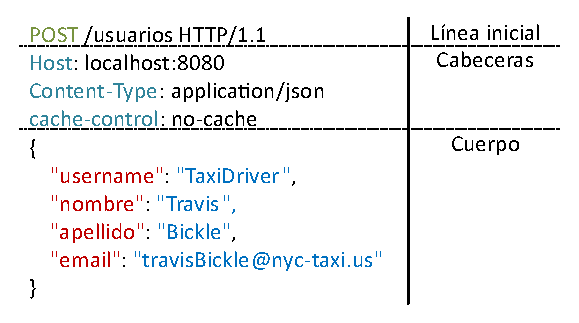
\includegraphics[width=0.8\linewidth]{images/http/httpRequest.eps}
    \end{center}
\end{frame}

\begin{frame}[c,fragile]
    \frametitle{HTTP Response}
    \begin{center}
        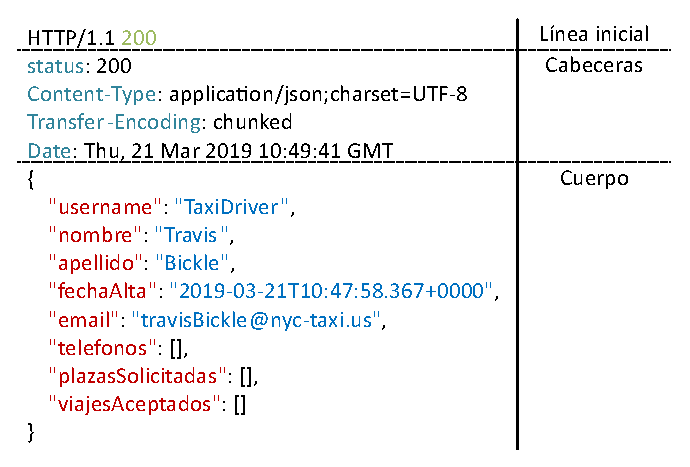
\includegraphics[width=0.8\linewidth]{images/http/httpResponse.eps}
    \end{center}
\end{frame}

\section{JSON}

\begin{frame}[c]
    \frametitle{Formato de intercambio JSON}
    \begin{center}
        \includegraphics[width=\linewidth]{images/http/enterpriseArchitectures02.eps}
    \end{center}
\end{frame}

\begin{frame}[c]
    \frametitle{Formato de intercambio JSON}
    \begin{block}{JSON}
        \emph{JSON (JavaScript Object Notation)} es un formato ligero de intercambio de datos fácilmente comprensible por humanos y fácilmente procesable por máquinas.
    \end{block}
\end{frame}

\begin{frame}[c,fragile]
    \frametitle{Gramática JSON}
\begin{verbatim}
    <json> ::= <object> | <array>
    <object> ::= {} | 
                 {(<string>:<value>,)* <string>:<value>}
    <value>  ::= <string> | <number> | <object> | 
                 array | true | false | null
\end{verbatim}
\end{frame}


\section{Creación de una API REST sobre HTTP}

\begin{frame}[c]
    \frametitle{API REST}
    \begin{center}
        \includegraphics[width=\linewidth]{images/apiRest/enterpriseArchitectures(api).eps}
    \end{center}
\end{frame}

\begin{frame}[c]
	\frametitle{Responsabilidades del Controlador HTTP}
	\begin{enumerate}[<+->]
        \item Atender las peticiones HTTP de los clientes.
        \item Convertir datos de HTTP al lenguaje que corresponda (\emph{unmarshalling}).
        \item Validar las peticiones de los clientes.
        \item Convertir las respuestas a una respuesta HTTP adecuada.
        \item Convertir los resultados a datos HTTP (\emph{marshalling}).
	\end{enumerate}
\end{frame}

\subsection{Identificación de recursos}

\begin{frame}[c]
    \frametitle{Creación de una API REST}
    \begin{enumerate}[<+->]
        \item Decidir qué elementos del \emph{domain model} se expondrán como \emph{recursos}.
        \item Exponer los \emph{aggregate roots} como colecciones.
        \item Exponer las partes internas de un \emph{aggregate roots} como elementos subordinados a un aggregate root.
        \item Exponer las operaciones de negocio que no corresponda a operaciones CRUDs básicas o parametrizadas como controladores, asociados al recurso que corresponda.
        \item Asignar una URI para cada recurso.
        \item Decidir qué verbos HTTP son aplicables a cada respuesta.
        \item Decidir los posibles parámetros de entrada a cada petición.
        \item Decidir las posibles respuestas a cada petición.
    \end{enumerate}
\end{frame}

\begin{frame}[c]
    \frametitle{Identificación de Recursos REST}
    \begin{enumerate}[<+->]
        \item Las colecciones de \emph{aggregates roots} se identifican con sustantivos en plural asociados a la raíz de la organización (\texttt{http://carsharing.es/viajes}).
        \item Las instancias de un \emph{aggregates roots} se identifican añadiendo el identificador de la instancia tras la URI asociado al \emph{aggregate root}
            (\texttt{/viajes/\{viajeId\}}).
        \item Los partes internas de un \emph{aggregate} se exponen siguiendo las mismas reglas, utilizando la URI del \emph{aggregate root} como prefijo (\texttt{/viajes/\{viajeId\}/conductor}).
        \item La regla anterior se aplica recursivamente a las partes internas de las partes internas de un aggregate (\texttt{/viajes/\{viajeId\}/conductor/vehiculos/}).
        \item Las operaciones no CRUD sobre un recurso se especifican como verbos tras la instancia del recurso al que se aplican (\texttt{/viajes/\{viajeId\}/cerrar}).
    \end{enumerate}
\end{frame}

\begin{frame}[c]
    \frametitle{Guía de Estilo para URIs REST}
    \begin{enumerate}[<+->]
        \item Utilizar \texttt{/} para indicar jerarquía o navegación por el modelo de dominio.
        \item No añadir una \texttt{/} final.
        \item Usar guiones \texttt{\-} para separar palabras.
        \item No usar guiones bajos.
        \item Usar sólo minúsculas.
        \item No referir ficheros, sino recursos.
        \item No utilizar URIs para distinguir operaciones CRUD.
        \item Utilizar parámetros para refinar operaciones CRUD (\texttt{/viajes?origen=Santander\&destino=Bilbao}).
    \end{enumerate}
\end{frame}

\subsection{Verbos HTTP y Recursos REST}

\begin{frame}[c]
    \frametitle{Verbos HTTP y Recursos REST}
    \begin{tabular}{ll} \hline
        GET    & Recupera un recurso. \\
        POST   & Añade un recurso (no identificado) a una colección. \\
        PUT    & Actualiza completamente (o añade) un recurso (identificado). \\
        PATCH  & Actualizar parcialmente un recurso. \\
        DELETE & Elimina un recurso. \\ \hline
    \end{tabular}
\end{frame}

\subsection{Códigos de Respuestas HTTP}

\begin{frame}[c]
    \frametitle{Códigos Respuesta HTTP}
    \begin{center}
        \begin{tabular}{ll}
            \hline
            200 & Ok         \\   
            201 & Created    \\  
            202 & Accepted   \\  
            204 & No content \\ 
            \hline
            400 & Bad request         \\
            401 & Unauthorized        \\   
            404 & Not Found           \\
            405 & Method Not Allowed  \\
            412 & Precondition Failed \\
            \hline
            500 & Internal Server Error \\
            501 & Not Implemented       \\
            \hline            
        \end{tabular}
    \end{center}
\end{frame}

\subsection{HATEOAS}

\begin{frame}[c]
    \frametitle{HATEOAS sobre JSON}
    \begin{center}
        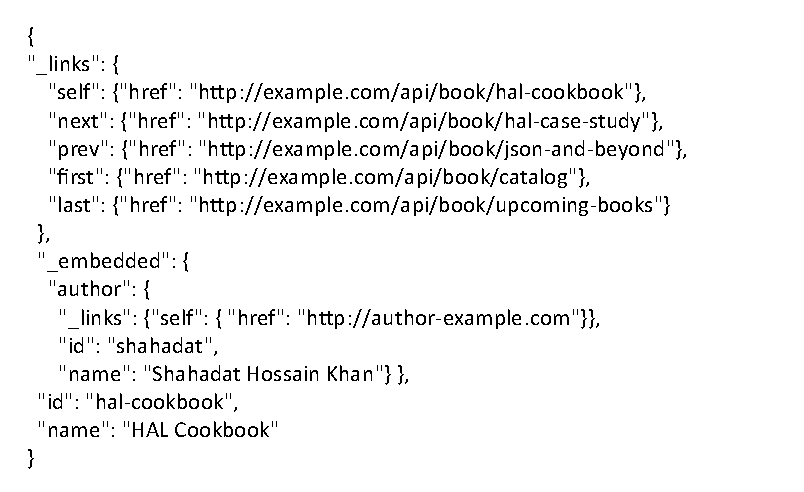
\includegraphics[width=\linewidth]{images/apiRest/hateoas.eps}
    \end{center}
\end{frame}




\subsection{Niveles de Adopción}

\begin{frame}[c]
    \frametitle{Niveles de Adopción REST}
    \begin{enumerate}[<+->]
        \item Utiliza el protocolo HTTP.
        \item Utiliza recursos REST.
        \item Utiliza verbos HTTP.
        \item Utiliza HATEOAS
    \end{enumerate}
\end{frame}

\section{Patrones de Servicio}

\subsection{Unit of Work}

\subsection{Data Transfer Object}

\section{Sumario}
%%
%%\begin{frame}[c]
%%    \frametitle{¿Qué tengo que saber de todo ésto?}
%%    \begin{enumerate}[<+->]
%%        \item
%%    \end{enumerate}
%%\end{frame}

\end{document} 